\subsection{Carte de développement}
La section \ref{sec:capteurAD8232} a détaillé les carectéristiques techniques du capteur. Maintenant, une foi le capteur délivre l'activité électrique via sa pin \mintinline{c++}{Output}, vers quelle carte de développement cette information sera finalement acheminée ?

Pour répondre à cette question, il est recommander de revoir les recommendations citées dans la section \ref{cahiercharges}. En effet, l'activité cardiaque doit être envoyée vers le WEB. Ce qui impose que la carte doit pouvoir se connecter à INTERNET. Une recherche comparative entre les différents boards éligibles tels que Arduino (avec ses variantes), STM32, ESP32 \ldots a été établie. Les critères de sélection retenus sont la connectivité, le prix et la disponibilité. Finalement, la carte ESP32 est celle qui répond mieux aux différentes contraintes. Elle offre plusieurs types de connectivités (WIFI, Bluetooth) avec un prix minimal.


\begin{figure}[H]
  \centering
  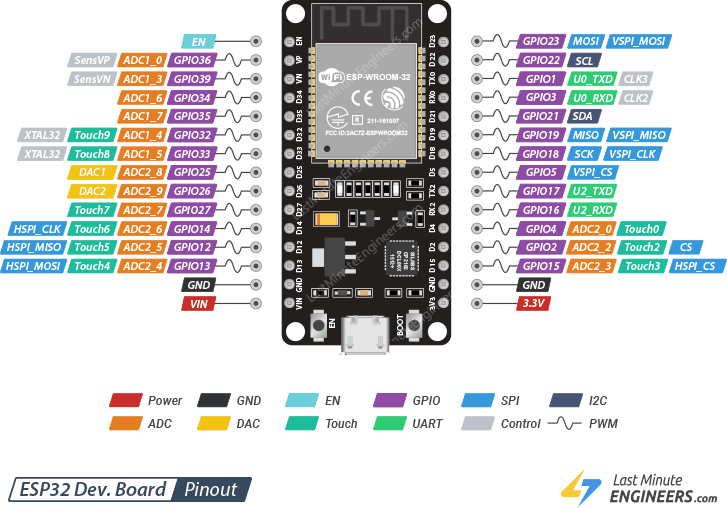
\includegraphics[scale=2]{imgs/ESP32-Pinout.png}
  \caption{Description de la carte de développement ESP32}
\end{figure}

L'ESP32 est un microcontroleur dont le constructeur est \textit{Espressif}. Ce constructeur a développé tout un système temps réel (FreeRTOS) pour ce microcontroleur. C'est pourquoi il est bien adapté aux applications temps réel et IoT. Il est caractérisé principalement par :
\begin{itemize}
  \item CPU : Xtensa double-cœur (ou simple-cœur), microprocesseur LX 32 bits, fonctionnant à 160 ou 240 MHz et fournissant jusqu'à 600 DMIPS, avec un
  coprocesseur ultra basse consommation (ULP)
  \item Mémoire : 520 KiO SRAM
  \item Connectivité sans-fil : Wi-Fi : 802.11 b/g/n;
  Bluetooth : v 4.2 BR/EDR et BLE jusqu'à v 5.0 et v 5.1
  \item 10 $\times$ capteurs de touché
  \item 4 $\times$ SPI
  \item 2 $\times$ interfaces I²S
  \item 2 $\times$ interfaces I²C
  \item 3 $\times$ UART
  \item interface MAC Ethernet avec DMA dédié et support du protocole de temps précis IEEE 1588
  \item Bus de données CAN 2.0
  \item Moteur PWM
\end{itemize}